
% The subsections written are only suggestions, to display how sections and subsections may look for your thesis

\section{About this report}
This report is a summary of work done in the course IP502122 - Specialization Project, undertaken in the autumn of 2024 at NTNU in Ålesund as a part of my master's degree in Product and Systems Engineering. The specialization project is intended as an introduction and "head start" on my master's thesis next semester. As such, the work done here is used in large part as a jumping off point for later.

\section{Marine plastic pollution}
Plastic pollution in the oceans has been widely documented, however the amount of plastic currently in the ocean is uncertain. Jambeck et al.\cite{jambeck_plastic_2015} estimates that in 2010, somewhere between 4.8 and 12.7 million metric tons(MT) of plastic ended up in the ocean. According to the World Economic Forum\cite{world_economic_forum_top_2022}, there is between 75 and 199 million MT currently in the ocean. Around two thirds of all plastics that end up in the ocean are heavier than seawater \cite{isobe_fate_2022} meaning that they sink and either drift in the pelagic zone or end up on the seafloor as litter. Removing litter and plastic pollution on a large scale is difficult, removing it under many meters of ocean makes it much more difficult. 

It is undesirable to have plastic waste in the oceans. This is because of the health effects the plastics have on marine and terrestrial life. Two points are especially of note: microplastics and leeching. Microplastics are plastic particles smaller than 5mm. Leeching on the other hand, is the plastics' chemical interaction with the seawater surrounding them, leeching harmful chemicals into the water. \textbf{TODO: kilder for mikroplast og leeching skadelighet} For both of these issues, the best solution is to remove the litter. This is because plastics' general longevity. For example, Oluwoye et al. \cite{oluwoye_degradation_2023} found that polyethylene, commonly used as a coating for subsea structures, would take about 800 years to degrade on the ocean floor. Polyethylene is also used in many consumer- and industrially facing applications, for instance in plastic cannisters for liquids, boxes and crates for fishing or other industrial practices, or as plastic bags. 

\section{The Plan Sea Project}
The desire to deal with sub-surface marine plastic waste, i.e. litter both in the pelagic zone and on the seabed, was what sparked the Plan Sea project. Plan Sea is a student driven project at NTNU in Ålesund with the goal of finding, developing and testing a potential solution for removing sub-surface plastics. The project is at time of writing still in its early phases and ongoing. 

Since this is not a report focused on the Plan Sea project, the proposed solution arrived at in Plan Sea will not be discussed in detail. However, because of the relationship between this project and Plan Sea, it is necessary to describe the solution at a surface level. 

\subsection{The proposed solution}
The solution arrived at which is currently under development is an ROV-based solution with an unmanned tender-vessel on the surface. The ROV has a gripper attached and will navigate to find litter, grab it and pick it up. The surface vessel exists to provide the ROV with a greater lifting capacity. If the ROV was to lift purely under its own force, as is traditional for ROVs, the total amount of lifting force available would be limited by the vertical thrust available on the ROV. This would mean that either the ROV would have to have a very large amount of vertical thrust available relative to its size, or that the total lifting capacity would be very small. By connecting the ROV to the surface vessel with a winch and a lifting cable, it is possible to use the ROV to do fine-navigation to find and attach to litter, and then use the lifting force of a winch and the total buoyancy of the surface vessel for lifting heavier objects. Additionally, the solution is supposed to have an undersea basket for collection to avoid the ROV needing to do the surface-bottom roundtrip for each piece of waste. A sketch of the solution can be seen in \cref{fig:overview}.

\begin{figure}
	\centering
	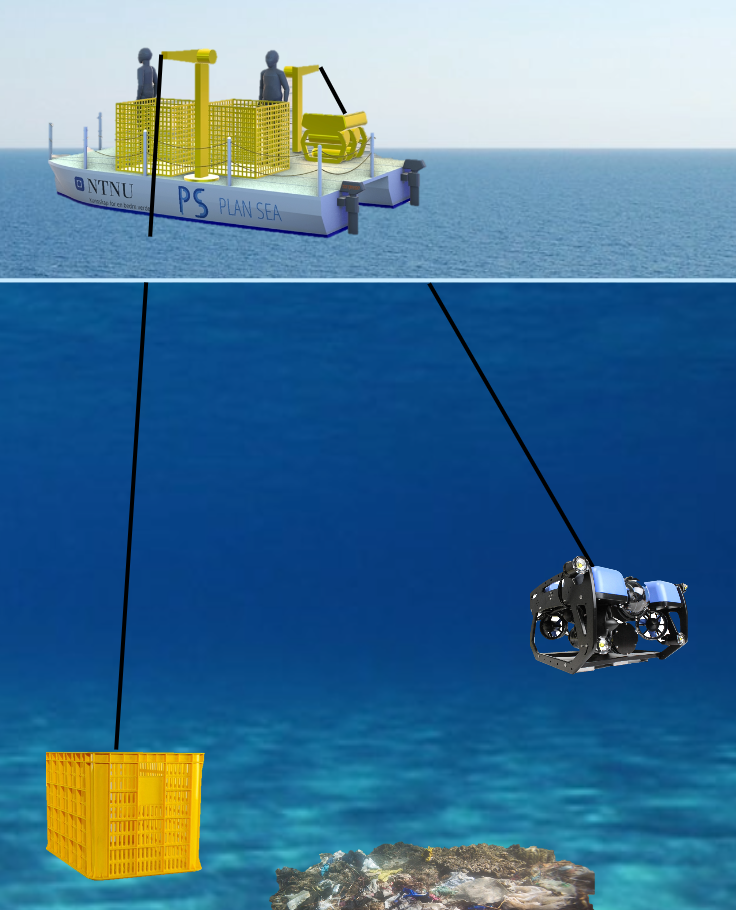
\includegraphics[width=0.45\textwidth]{overview}
	\caption{A sketch of the proposed solution for Plan Sea showing a surface vessel, a tethered ROV and a collection basket}
	\label{fig:overview}
\end{figure}

Using this solution allows for completely ignoring the buoyancy of the ROV, unlike traditional ROVs. Traditional ROVs are generally designed to be neutrally buoyant, meaning that they neither sink nor float, but keep their vertical position in water once placed there. Since the Plan Sea ROV will be attached to a cable to the surface vessel at all times, it can instead hang from the cable. This means that it's possible to attach larger grippers, more battery capacity, more detection/lighting/navigation equipment, and otherwise allows for pretty much whatever is desired to be done to the ROV. Additionally, since the ROV doesn't need to provide vertical thrust, it is much easier to not disturb the seabed which will provide a clearer view for detection equipment based on visible or near-visible light. However, having a non-buoyant ROV does come with some drawbacks.

One drawback of this solution is that it will switch between two operating modes, searching/grabbing and lifting, increasing the complexity of the system. Another drawback is that as the ROV is hanging from the cable, it creates a coupled system consisting of the surface vessel and the ROV, and necessitates the two moving together as one unit. 

This project is focusing on how to control the two units as one. 

\section{Control systems}
A control system commands and regulates the behaviour of other systems automatically. For this project in particular, the control system will be in charge of maintaining and changing positions of the surface vessel and the ROV. A simplified function block diagram of the total system can be seen in \cref{fig:fbd}. The goal of the simulator is to function as a drop-in replacement for the vessel, local controllers and environmental impact. This makes it so that the development can happen digitally to then be quickly deployed in the real-world. 

\begin{figure}
	\centering
	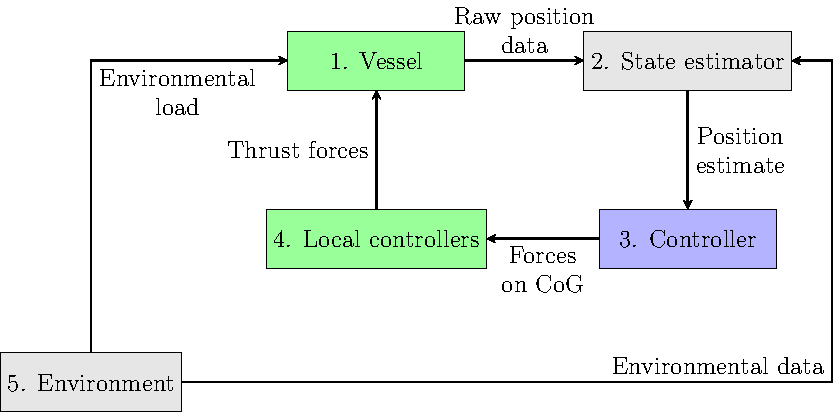
\includegraphics[width=0.8\textwidth]{control-fbd}
	\caption{A simplified function block diagram of the total system. Grey blocks are not currently implemented, green blocks are simulated and blue is for the controller which is system-agnostic}
	\label{fig:fbd}
\end{figure}


\subsection{Considerations because of a coupled system}
In the marine sector, dynamic positioning (DP) is commonly used. DP allows for a vessel to maintain a position or a course automatically despite external effects. This is used for example for offshore supply vessels which need to stay stationary relative to an anchored platform to allow loading and offloading of supplies. DP is also used for applications such as laying subsea fiberoptic cables, where maintaining correct speed and course is important to avoid damaging the cables. For the Plan Sea project too, a DP system is necessary because it consists of vessels that need to maintain specific positions at sea with wind, wave and current forces affecting the vessels

Normally a DP system only considers one vessel, however for the Plan Sea project it has to be more comprehensive than that because the two vessels are coupled. This is all further discussed in \cref{sec:math}

\subsection{The need for rapid prototyping}
Rapid prototyping is a concept used increasingly as time goes on. The point of rapid prototyping is to create some simulated environment in which you can test and iterate on a solution until it is acceptable, before putting materials and resources into building and implementing the solution in the real world. 

For my purposes, rapid prototyping will allow me to experiment with control system tuning and variables without having to deploy the full-scale vessel every time. Ideally, the solution arrived at in the prototyping stage will be directly applicable to the full-scale version, which allows for rapid deployment and only some interfacing issues to solve in the field, rather than larger issues. \textbf{TODO: Omformuler det her}

\section{Problem description}
A simplified sketch from \cref{fig:overview} can be seen in \cref{fig:simple}. It shows the three main components of this system: The surface vessel, the ROV, and the tether between them. It also shows the forces in the tether. As the tether holds the ROV up, the tether pulls the surface vessel down. This follows from Newton's second law of motion. The figure also shows the coupled nature of the system, since the tether will be taut at all times, both vessels will

\begin{figure}
	\centering
	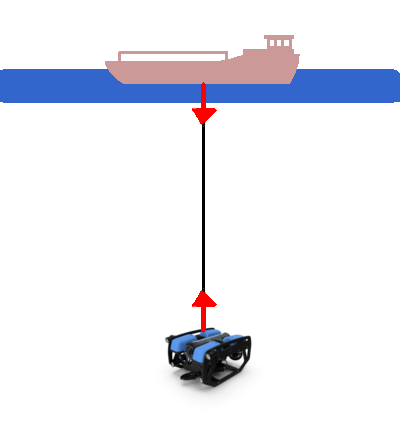
\includegraphics[width=0.5\textwidth]{simplified-overview}
	\caption{A simplified sketch of the problem, forces experienced by each vessel are shown in red.}
	\label{fig:simple}
\end{figure}

In \cref{fig:angled} two scenarios are shown at the same time, one where the ROV is hanging straight below the surface vessel and another where it is at an angle. The result is that the ROV is not at a constant height. If we imagine a desired elevation above the seafloor is constant, then either the ROV needs to have more tether payed out and provide lift through its own thrusters, or the surface vessel needs to move to allow the ROV to hang perpendicular to the surface of the sea. If more tether was to be payed out, if the system then stabilizes with the ROV at the lowest possible point, it is possible the ROV might collide with the seabed. The ideal solution then becomes that the surface vessel follows the ROV, or the ROV only operates within a given area of operations directly underneath of the surface vessel. 

\begin{figure}
	\centering
	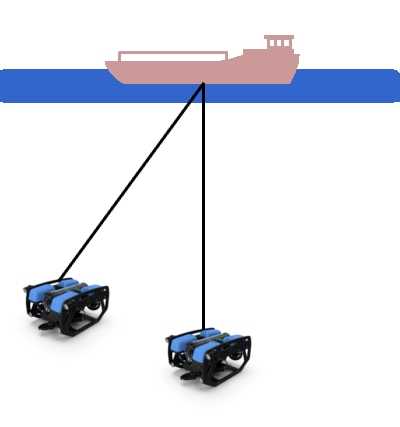
\includegraphics[width=0.5\textwidth]{angled}
	\caption{The ROV is hanging from the same point on the surface vessel with an equal tether. Note how the height of the ROV has changed because the tether has stayed the same}
	\label{fig:angled}
\end{figure}

Further, this non-perpendicular arrangement will lead to tangential forces, shown in \cref{fig:angled-force}. The forces will of course be mirrored on the vessel's end, but this has been omitted from the figure for clarity. The horizontal force the tether imparts on the ROV will act as a restoring force, trying to move it back to be perpendicular to the surface vessel. The surface vessel likewise will experience a pull towards the ROV. 

\begin{figure}
	\centering
	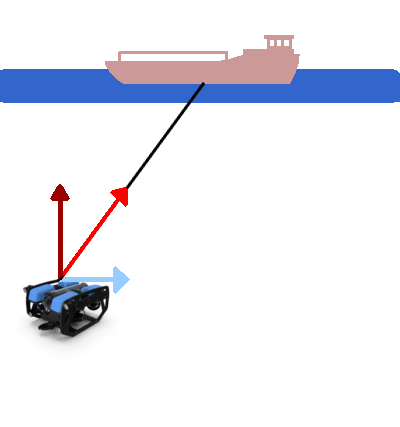
\includegraphics[width=0.5\textwidth]{angled-component}
	\caption{The component forces on the ROV resulting from an angled lift, decomposed}
	\label{fig:angled-force}
\end{figure}

Because these two vessels are connected and so dependent on each other's positions, the control systems of each need to take this into account. Probably, the simplest solution will be to have one large control system handling both, or alternately having one of the vessels take a leading part and the other attempt to follow.  

\section{Statement of intent}
For this project I want to create a simulation which is able to quantify the effects that the parts of the system have on each other. I want to be able to measure the tension in the wire, the force exerted by the vessels, how well the vessels follow each other or orders given and influence from the environment. The goal of this simulation is to be used as a future design tool for finalizing design of the Plan Sea vessel, its control systems, as well as defining operational criteria. 